
    \item A wheel of radius \( R \) and mass \( M \) is placed at the bottom of a fixed step of height \( R \) as shown in the figure. A constant force is continuously applied on the surface of the wheel so that it just climbs the step without slipping. Consider the torque \( \tau \) about an axis normal to the plane of the paper passing through the point \( Q \). Which of the following options is/are correct?
        \begin{tasks}(1)
            \task If the force is applied at point \( P \) tangentially then \( \tau \) decreases continuously as the wheel climbs
            \task If the force is applied normal to the circumference at point \( X \) then \( \tau \) is constant
            \task If the force is applied normal to the circumference at point \( P \) then \( \tau \) is zero
            \task If the force is applied tangentially at point \( S \) then \( \tau \neq 0 \) but the wheel never climbs the step
        \end{tasks}


\begin{center}
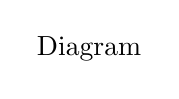
\begin{tikzpicture}
\node {Diagram};
\end{tikzpicture}
\end{center}